\section{The Origins of Software Ecosystems}
\label{INT:sec:origin}
Today, \emph{software ecosystems} are considered an important domain of study within the general discipline of \emph{software engineering}. This section describes its origins, by summarising the important milestones that have led to its emergence.
\fig{INT}{milestones} depicts these milestones chronologically.

\begin{figure}[htbp]
   \centering
   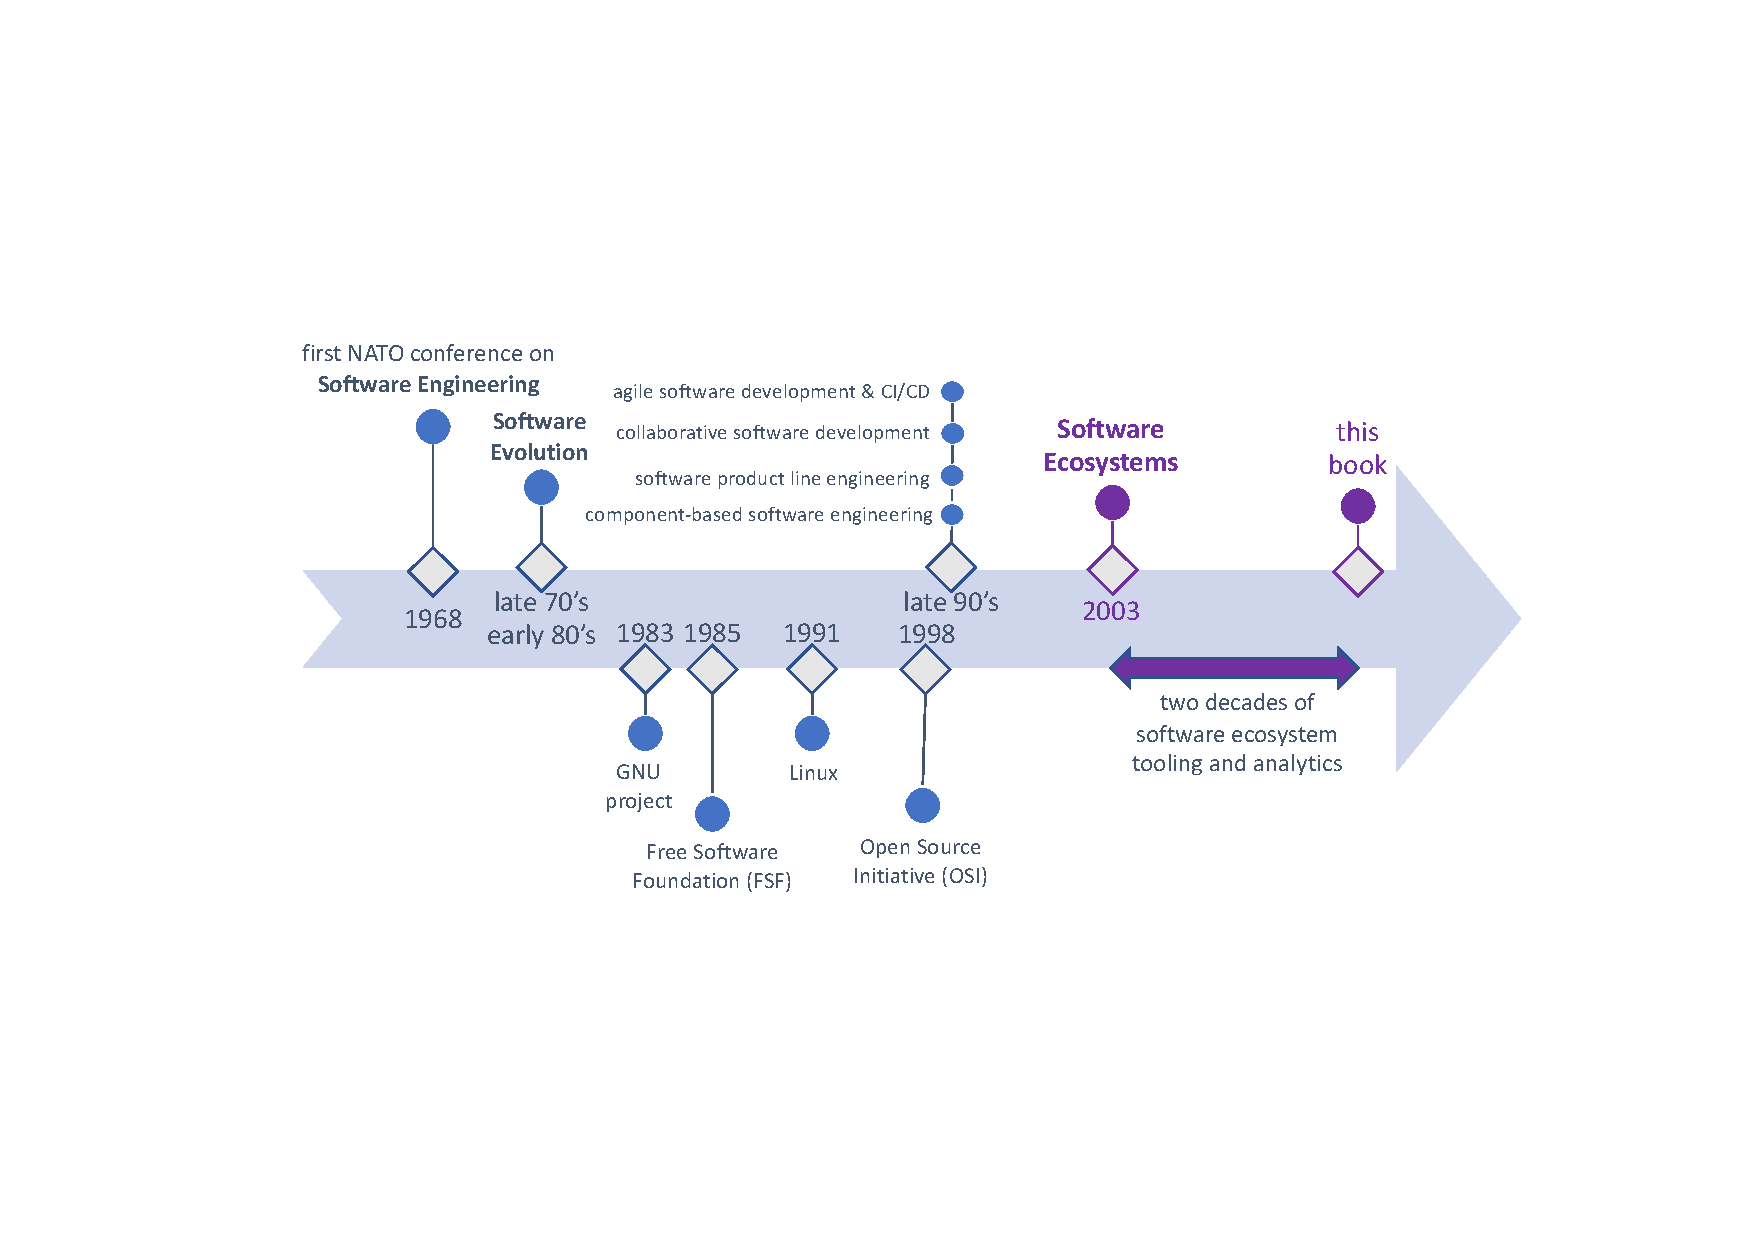
\includegraphics[width=\textwidth]{SECO-history.pdf} % requires the graphicx package
   \caption{Milestones that contributed to the domain of research (analytics) and development (tooling) of \emph{software ecosystems}}
   \label{INT:fig:milestones}
\end{figure}

The software engineering discipline emerged in 1968 as the result of a first international conference~\cite{Naur1969}, sponsored by the NATO Science Committee, based on the realisation that more disciplined techniques, engineering principles, and theoretical foundations were urgently needed to cope with the increasing complexity, importance, and impact of software systems in all sectors of economy and industry.
Even the key idea of \emph{software reuse}~\cite{Krueger1992,Frakes2005}, which suggests to reduce time-to-market, cost, and effort when building software, while at the same time increasing reuse, productivity, and quality, is as old as the software engineering discipline itself.
During the aforementioned conference, Malcolm Douglas McIllroy proposed to face increasing software complexity by building software through the reuse of high-quality software components~\cite{McIllroy1968}.

In the late seventies, awareness increased that the development of large-scale software needs to \emph{embrace change} as a key aspect of the development process~\cite{Yau1978}.
This has led Manny Lehman to propose the so-called laws of \emph{software evolution}, focusing on how industrial software systems continue to evolve after their first deployment or public release~\cite{Lehman1976,Lehman1980,Lehman1980a}.
The software evolution research domain is still thriving today~\cite{Mens2008,Mens2014-ESS}, with two dedicated annual conferences: the IEEE International Conference on Software Maintenance and Evolution (ICSME) and the IEEE Software Analysis, Evolution and Reengineering Conference (SANER).

Another important factor having contributed to the popularity of software ecosystems is the emergence and ever-increasing importance of \emph{free software} and \emph{open source software} (OSS) since the early eighties, partly through the creation of the GNU project\footnote{\url{https://www.gnu.org}} in 1983 and the Free Software Foundation (FSF) in 1985 by Richard Stallman, as well as the creation of the Linux operating system in 1991.
Strong open source advocates such as Eric Raymond~\cite{Raymond1999} further contributed to the popularity through the creation of the Open Source Initiative (OSI) in 1998, and by contrasting cathedral-style closed development process models with the bazaar-style open development process models for open source and free software in which the code is publicly developed over the Internet.
This bazaar-style model evolved into geographically distributed \emph{global software development}~\cite{Grinter1999,Herbsleb2001} models, supported by the immensely popular \emph{social coding platforms}~\cite{Dabbish2012} such as GitHub, GitLab, Gitea and BitBucket.

In parallel, the importance of software reuse in the late nineties gave rise to additional subfields of software engineering such as the domain of \emph{component-based software engineering}~\cite{Szyperski1997,Kozaczynski1998CBSE}, focusing on methods and principles for composing large systems from loosely-coupled and independently-evolving software components.
Around the same time it was joined by another subfield, called \emph{software product line engineering}~\cite{Weiss199SPLE,Clements1999}, which explicitly aims to enable developing closely-related software products using a process modelled after product line manufacturing, separating the \emph{domain engineering} phase of producing reusable software artefacts that are common the product family, from the \emph{application engineering} phase that focuses on developing concrete software applications that exploit the commonalities of the reusable artefacts created during the domain engineering phase.
Software product lines have allowed many companies to reduce costs while at the same time increasing quality and time to market, by providing a product line platform and architecture that allows to scale up from the development and maintenance of individual software products to the maintenance of entire families of software products. However, these product families still remain within the organisational boundaries of the company.

Around the same time, the lightweight and iterative process models known as \emph{agile software processes} started to come to the forefront, with a user-centric vision requiring adaptive and continuous software change.
Different variants, such as Scrum \cite{Schwaber1997} and eXtreme Programming (XP) \cite{Beck1999}, led to the foundation of the Agile Alliance and the creation of the agile manifesto \cite{beck2001manifesto}.
In support of agile software processes, various development practices and tools for \emph{continuous integration and delivery} (CI/CD) emerged later on in the decade.

Since the seminal 2003 book by Messerschmitt and Szyperski~\cite{messerschmitt2003software}, \emph{software ecosystems} have become an active topic of research in software engineering.
As argued by Jan Bosch~\cite{Bosch2009,Bosch2010}, software ecosystems expand upon software product lines by allowing companies to cross the organisational boundaries and make their software development platforms available to third parties that, in turn, can contribute to the popularity of the produced software through externally developed components and applications.
The key point of software ecosystems is that software products can no longer be considered or maintained in isolation, since they have become heavily interconnected.


\section{Perspectives and Definitions of Software Ecosystems}
\label{INT:sec:definition}

Messerschmitt and Szyperski \cite{messerschmitt2003software} were arguably among the first to use the term \emph{software ecosystem}, and defined it rather generically as \emph{``a collection of software products that have some given degree of symbiotic relationships.''} Since then, the research literature has provided different definitions of software ecosystems, from many different perspectives.

From an \textbf{ecological perspective}, several researchers have tried to exploit the analogy between software ecosystems and ecological ecosystems.
The term software ecosystem quite obviously originates from its ecological counterpart of biological ecosystems that can be found in nature, in a wide variety of forms (\eg rainforests, coral reefs, deserts, mountain zones, and polar ecosystems).
In 1930, Roy Clapham introduced the term \emph{ecosystem} in an ecological context to denote the \emph{``physical and biological components of an environment considered in relation to each other as a unit''}~\cite{Willis1997}.
These components encompass all living organisms (e.g., plants, animals, micro-organisms) and physical constituents (e.g., light, water, soil, rocks, minerals) that interact with one another in a given environment.
Dunghana \etal \cite{Dhungana2013} compared the characteristics of natural and software ecosystems. Mens \cite{Mens2015} provided a high-level historical and ecological perspective on how software ecosystems evolve.
Moore \cite{Moore1993} and Iansiti and Levien \cite{Iansiti2004} focused on the analogy between business ecosystems and ecology.

From an \textbf{economic and business perspective}, Jansen \etal \cite{Jansen2009-ICSE} provide a more precise definition: \emph{``a set of businesses functioning as a unit and interacting with a shared market for software and services, together with the relationships among them.''} In a similar vein,
Bosch \etal~\cite{Bosch2009} say that a software ecosystem \emph{``consists of a software platform, a set of internal and external developers and a community of domain experts in service to a community of users that compose relevant solution elements to satisfy their needs.''}
Hanssen~\cite{Hanssen2012} defines it as \emph{``a networked community of organizations, which base their relations to each other on a common interest in a central software technology.''}
An excellent entry point to this business-oriented viewpoint on software ecosystems is the book edited by Jansen \etal~\cite{Jansen2013book}.
In contrast, the chapters in the current book focus mostly on the complementary technical and social perspectives.

From a more \textbf{technical perspective}, the focus is on technical aspects such as the software tools that are being used (\eg version control systems, issue and bug trackers, social coding platforms, integrated development environments, programming languages) and the software artefacts that are being used and produced (\eg source code, executable code, tests, databases, documentation, trace logs, bug and vulnerability reports).
Within this technical perspective, Lungu \cite{Lungu2008} defined a software ecosystem as \emph{``a collection of software projects that are developed and evolve together in the same environment''.}
The notion of \emph{environment} can be interpreted rather broadly.
The environment can correspond to a software-producing organisation, including the tools and libraries used by this organisation for developing its software projects, as well as the clients using the developed software projects.
It can correspond to an academic environment, composed of software projects developed and maintained by students and researchers in research units.
It can also correspond to an entire OSS community consisting of geographically dispersed project collaborators focused around similar philosophies or goals.

From a \textbf{social perspective}, the focus is on the social context and network structure that emerges as a result of the collaboration dynamics and interaction between the different contributors to the projects that belong to the software ecosystem.
This social structure is at least as important as the technical aspects, and includes the various stakeholders that participate in the software ecosystem, such as developers, end users, project managers, analysts, designers, software architects, security specialists, legal consultants, clients, QA teams, and many more.
\chap{EMO} focuses on these social aspects from an emotion analysis viewpoint.

Manikas \cite{ManikasHansen2013} combined all these perspectives into a single all-encompassing definition of a software ecosystem as \emph{``the interactions of a set of actors on top of a common technological platform that results in a number of software solutions or services. Each actor is motivated by a set of interests or business models and connected to the rest of the actors and the ecosystem as a whole with symbiotic relationships, while the technological platform is structured in a way that allows the involvement and contribution of the different actors.''}

%(Terminology of "registry" / "index")
%(Notion of reusable assets / components / dependencies )


\section{Examples of Software Ecosystems}
\label{INT:sec:SECO-examples}

Following the wide diversity of definitions of software ecosystem, the kinds of software ecosystems that have been studied in recent research are equally diverse.
An interesting entry point into how the research literature on software ecosystems has been evolving over the years are the many published systematic literature reviews, such as \cite{Barbosa2011, ManikasHansen2013, Manikas2016, Seppanen2017, Burstrom2022}.

Without attempting to be complete, \tab{INT}{secokinds} groups into different categories some of the most popular examples of software ecosystems that have been studied in the research literature. These categories are not necessarily disjoint, since software ecosystems tend to contain different types of components that can be studied from different viewpoints.

% Requires the booktabs if the memoir class is not being used
\begin{table}[htbp]
   \centering
   %\topcaption{Table captions are better up top} % requires the topcapt package
   \caption{Categories of software ecosystems}
   \label{INT:tab:secokinds}
   \begin{tabular}{p{2.2cm}p{3.3cm}p{2.8cm}p{2.7cm}}
      \toprule
      Category                                                  & Examples                                                                                                                                         & Components                                                                             & Contributors                                                                 \\
      \midrule
      digital platform                                          & mobile app stores, integrated development environments                                                                                           & mobile apps; software plug-ins or extensions                                           & third-party app or plug-in developers and their users                        \\\\
      social coding platform                                    & \sourceforge, \github, \gitlab, \gitea, \bitbucket                                                                                               & software project repositories                                                          & software project contributors                                                \\\\
      component-based software ecosystem                        & software library registries (\eg CRAN, \npm, RubyGems, PyPi, Maven Central), OS package registries (\eg Debian packages, Ubuntu package archive) & interdependent software packages                                                       & consumers and producers of software packages and libraries                   \\\\
      automation, containerisation and orchestration ecosystems & \dockerhub, Kubernetes, Ansible~Galaxy, Chef~Supermarket, Puppetforge                                                                            & container images, configuration and orchestration scripts, workflow automation scripts & creators and users of automation, containerisation and orchestration systems \\\\
      communication-oriented ecosystem                          & mailing lists, \stackoverflow, Slack                                                                                                             & e-mail threads, questions, answers, messages, posts, \ldots                            & programmers, developers, end-users, researchers                              \\\\
      OSS communities                                           & Apache Software Foundation, Linux Foundation                                                                                                     & OSS projects                                                                           & community members, code contributors, project maintainers, end users         \\\\
      \bottomrule
   \end{tabular}
\end{table}

The remaining subsections provide more details for each category, illustrating the variety of software ecosystems that have been studied, and providing examples of well-known ecosystems and empirical research that has been conducted on them.

\subsection{Digital Platform Ecosystems}
\label{INT:sec:digitalplatforms}

Hein \etal~\cite{Hein2020} define a \emph{digital platform ecosystem} as a software  ecosystem that \emph{``comprises a platform owner that implements governance mechanisms to facilitate value-creating mechanisms on a digital platform between the platform owner and an ecosystem of autonomous complementors and consumers''}.
This is in line with the previously mentioned definition by Bosch \etal~\cite{Bosch2009} that a software ecosystem \emph{``consists of a software platform, a set of internal and external developers and a community of domain experts in service to a community of users that compose relevant solution elements to satisfy their needs.''}

Well-known examples of digital platform ecosystems are the \emph{mobile software ecosystems} provided by companies such as Microsoft, Apple and Google.
The company owns and controls an \emph{app store} as a central platform to which other companies or individuals can contribute apps to this platform, which in turn can be downloaded and installed by mobile device users.
The systematic mapping studies by de Lima Fontao \etal \cite{deLimaFontao2015} and \cite{Steglich2019} report on the abundant research that has been conducted on these mobile software ecosystems.
%Given that research on mobile apps (especially Android apps) is extremely prolific, we do not attempt to summarise it here, as this would lead us to far for this introductory chapter.
%SOME REFS:\cite{Mankad,1-100,1-102, 2-011,2-201,2-059,1-089,2-067,2-068,2-085,2-089}\cite{Hyrynsalmi2014, mcdonnell2013empirical, bavota2014impact, Lyu2017, yang2018android, huang2018understanding, he2018understanding, understandingfic, thung2020automated}
%Abstract deLimaFontao2015: The development of mobile applications around a central software platform has been impacting the software industry. Software solutions are collaboratively built within a dynamic market, often requiring adaptation of software development processes. This trend has been broadly studied as Software Ecosystem (SECO) - in the mobile platform domain, named as Mobile Software Ecosystem (MSECO). In this paper, we share the results of a systematic mapping study on the MSECO field that analyzed 28 papers identified as relevant to answer our research questions. The results indicate the growing interest in this research field as well as the main software platforms and trending topics. We confirmed the three main MSECOs as Android (Google), iOS (Apple) and Windows Phone (Microsoft). We observed the more investigated area is mobile app development. Finally, we highlighted the main benefits: the attracting and supporting developers, then helping developers to learn and create content and the app store that allows selling and buying processes.
%Absrtract Steglich2019: Software Ecosystems are comprised of a technology platform, business models, internal and external developers, and engaging users. The popularity of smartphones brought along the mobile software ecosystems, such as iOS and Android, which are composed of a platform, a community of users and developers, mobile applications, and online application store, and evangelists that often promote the ecosystem. Given the recent nature of the topic, this paper aims to revisit the state-of-the-art through a systematic literature mapping. We found 63 publications on the topic of mobile software ecosystems that were categorized by year (almost 50% of the publications are from 2015 and on), by author (a few collaboration clusters were identified), and by the mobile ecosystems characteristics (most publications discuss business or technical aspects) and elements (applications and the platform are the most discussed topics followed by the developers and the users). Our results provide an up-to-date map of the topic for those interested in mobile software ecosystems.

Any software system that provides a mechanism for third parties to contribute plug-ins or extensions that enhance the functionalities of the system can be considered as a digital software ecosystem. Examples of these are configurable text editors such as Emacs and Vim, and integrated software development environments (IDEs) such as IntelliJ IDEA, VS Code, NetBeans and Eclipse.
The latter ecosystem in particular has been the subject of quite some research on its evolutionary dynamics (\eg \cite{MensRamil2008-ICSM,Businge:SQJ:2015,Businge2012Survival,Businge2013CSMR,Businge:Eclise:saner:2019,Kawuma:ICPC:2016,2-236, AbouKhalil2021, Nugroho2021}).
These examples show that digital platform ecosystems are not necessarily controlled by a single company.
In many cases, they are managed by a consortium, foundation or open source community.
For example, NetBeans is controlled by the Apache Foundation, and Eclipse is controlled by the Eclipse Foundation.

Another well-known digital platform ecosystem is WordPress, the most popular content management system in use today, which features a plugin architecture and template system that enables third parties to publish themes and extend the core functionality.
Um \etal \cite{Um2022WordPress} presented a recent study of this ecosystem.
Yet another example is OpenStack, an open source cloud computing platform involving more than 500 companies.
This ecosystem has been studied by several researchers (\eg \cite{2-236,Teixeira2017,Foundjem:2022wx,Zhang2022}).
%Abstract from Teixeira2017: Much research that analyzes the evolution of a software ecosystem is confined to its own boundaries. Evidence shows, however, that software ecosystems co-evolve independently with other software ecosystems. In other words, understanding the evolution of a software ecosystem requires an especially astute awareness of its competitive landscape and much consideration for other software ecosystems in related markets. A software ecosystem does not evolve in insulation but with other software ecosystems. In this research, we analyzed the OpenStack software ecosystem with a focal perspective that attempted to understand its evolution as a function of other software ecosystems. We attempted to understand and explain the evolution of OpenStack in relation to other software ecosystems in the cloud computing market. Our findings add to theoretical knowledge in software ecosystems by identifying and discussing seven different mechanisms by which software ecosystems mutually influence each other: sedimentation and embeddedness of business relationships, strategic management of the portfolio of business relationships, firms values and reputation as a partner, core technological architecture, design of the APIs, competitive replication of functionality and multi-homing. Research addressing the evolution of software ecosystem should, therefore, acknowledge that software ecosystems entangle with other software ecosystems in multiple ways, even with competing ones. A rigorous analysis of the evolution of a software ecosystem should not be solely confined to its inner boundaries.


\subsection{Component-based Software Ecosystems}
\label{INT:sec:CBSECO}

A very important category of software ecosystems are so-called \emph{component-based software ecosystems}.
They constitute large collections of reusable software components, which often have many interdependencies among them~\cite{Abate2009}.
Empirical studies on component-based software ecosystems tend to focus on the technicalities of dependency-based reuse, which differentiates them from studies on digital platform ecosystems which have a more business-oriented and managerial focus.

As explained in \sect{INT}{origin}, the idea of building software by reusing existing software components is as old as the software engineering discipline itself, since it was proposed by McIllroy in 1968 during the very first software engineering conference~\cite{McIllroy1968}.
The goal was to reduce time-to-market, cost and effort when building software, while at the same time increasing reuse, productivity and quality.
This has given rise to a very important and abundant subfield of software engineering that is commonly referred to as component-based software engineering.
Despite the large body of research in this field (\eg \cite{Caldiera1991,Krueger1992,Szyperski1997}) it was not able to live up to its promises due to a lack of a standard marketplace for software components, combined with a lack of proper component models, terminology, and scalable tooling \cite{Kotovs2009}.
All of this has changed nowadays, probably due to a combination of the increasing popularity of OSS and the emergence of affordable cloud computing solutions.
\coen{Contemporary success stories (packages, libraries) seem to have done away with component models. Does the literature still consider these as instances of component-based software engineering?}
\tom{@coen: Probably not, I have not seen this in the litterature, but I did not check recent literature on component-based software engineering. Should we? (Here is a recent reference, but I do not have access to it: \cite{Gholamshahi2019}}

Among the most important success stories of component-based software ecosystems are undoubtedly the
many interconnected \emph{software packages} for OSS operating systems such as the GNU Project since 1983, Linux since 1991, Debian since 1993 (\eg \cite{Abate2009,gonzalez2009macro,debsources-esem-2014,Claes2015,Claes2018}) and Ubuntu since 2004.
They come with associated \emph{package management systems} (or \emph{package managers} for short) such as DPKG (since 1994) and APT (since 1998), which are systems that automate the process of selecting, installing (or removing), upgrading and configuring of those packages.
Package managers typically maintain a database of software dependencies and version information to prevent software incompatibilities.

%\coen{Software libraries already existed before package manager for operating systems. I would not suggest a causal link. Perhaps it's better to introduce libraries as a second type of reusable components.}
%\tom{Done!}

Another popular type of ecosystems of reusable components are \emph{software libraries}. Software developers, regardless of whether they are part of an OSS community or software company, rely to a large extent on such reusable third-party \emph{software libraries}. These library ecosystems tend to come with their own specific package managers and package registries, and are available for all major programming languages. Examples include the CPAN archive network (created in 1995 for the Perl programming language, the CRAN archive network (created in 1997) and Bioconductor for the R statistical programming language)~\cite{German2013,Plakidas2017-JSS},
npm %(since 2010)
and Bower for JavaScript~\cite{cogo2021deprecation, abdalkareem2017developers,decan2018evolution,decan2018impact,decan2021back,zerouali2022impact}, %ahmed citeren, kth citeren
PyPI for Python~\cite{valiev2018ecosystem}, %(since 2003)
Maven (Central)~\cite{Benelallam2019,soto2021comprehensive,Ochoa2022-EMSE} for JVM-based languages such as Java and Scala,
Packagist for PHP,
RubyGems for Ruby~\cite{Kabbedijk2011,decan2021back,zerouali2022impact},
NuGet for the .NET ecosystem~\cite{Li2022-ICSE},
and the Cargo package manager and its associated crates registry for the Rust programming language~\cite{decan2018evolution,Schueller2022-Rust}.
Another example is the Robot Operating System (ROS), the most popular middleware for robotics development, offering reusable libraries for building a robot, distributed through a dedicated package manager \cite{Estefo2019,Pichler2019ROS,Kolak2020ROS}.


Decan \etal \cite{decan:emse:2019} studied and compared seven software library ecosystems for programming languages, focusing on the evolutionary characteristics of their package dependency networks.
They observed that library dependency networks tend to grow over time, but that some packages are more impactful than other.
A minority of packages are responsible for most of the package updates, a small proportion of packages accounts for most of the reverse dependencies, and there is a high proportion of fragile packages due to a high number of transitive dependencies.
This makes software library ecosystems prone to a variety of technical, dependency-related issues~\cite{decan2017empirical,abdalkareem2017developers,Claes2018,soto2021comprehensive}, licensing issues~\cite{2022:icsr:makari}, security vulnerabilities~\cite{decan2018impact,zerouali2022impact,Alfadel2021}, backward compatibility~\cite{decan2021what,decan2021back,bogart2021and}, and reliance on deprecated, obsolete or outdated components~\cite{cogo2021deprecation,decan2018evolution,zerouali2019formal,lauinger2018thou}.
Library ecosystems also face many social challenges, such as how to attract and retain contributors and how to avoid contributor abandonment \cite{Constantinou2017}.

%Smalltalk/Pharo: robbes2012developers, horadevelopersapievolution


\subsection{Web-based Code Hosting Platforms}

\begin{figure}
   \centering
   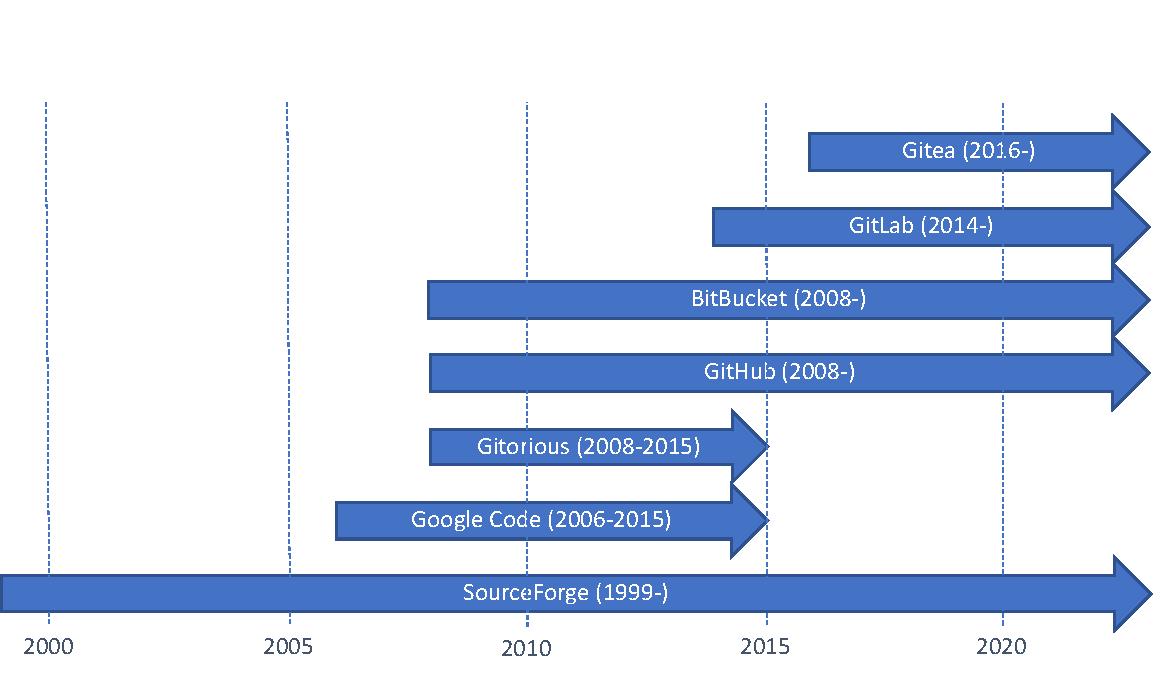
\includegraphics[width=\textwidth]{codehosting.pdf} % requires the graphicx package
   \caption{Historical overview of source code hosting platforms}
   \label{INT:fig:codehosting}
\end{figure}

The landscape of web-based code hosting platforms has seen many important changes over the last two decades, as can be seen in \fig{INT}{codehosting}.
\sourceforge was created in 1999 as a centralized web-based platform for hosting and managing the version history of free and OSS projects. It used to be a very popular data source for empirical research (\eg \cite{Howison2004,Robles2006, Koch2009,Nyman2011}). This is no longer the case today, since the majority of OSS projects have migrated to other hosting platforms.
Since 2006, Google ran a similar open source project hosting service, called Google Code, but it was closed down in January 2016. The same happened for Gitorious that ran from 2008 to 2015.

\github replaced Google Code as the most popular and largest hosting platform for open source (and commercial) software projects that use the git version control system. Other alternatives such as \bitbucket (also created in 2008) and \gitlab (created in 2014) and the likes are much less popular for hosting OSS projects. A relatively new contender in the field is \gitea, created in 2016 and funded by the Open Source Collective.
%For completeness we also mention Software Heritage that will be presented in detail in \chap{SWH}. Strictly speaking it is not a code hosting platform, but rather a code archival platform aiming to preserve software code in the very long term.

\github contains historical information about hundreds of millions of OSS repositories and has been the subject of many empirical studies focusing on different aspects \cite{Kalliamvakou2014}.
\github is claimed to be the first \emph{social coding} platform~\cite{Dabbish2012}, since it was the first hosting platform to provide a wide range of mechanisms and associated visualisations to increase collaboration by making socially significant information visible: watching, starring, commits, issues, pull requests and commenting.
Being an enabler of social coding, the social aspects in \github projects have been frequently studied~\cite{Tsay2014, padhye2014extcontrib}, including
communication patterns \cite{1-042},
collaboration through pull requests  \cite{Rahman:MSR:2014, Yu:MSR:2015, Gousios2016},
variation in contributor workload~\cite{Vasilescu2014},
gender and tenure diversity \cite{vasilescu2015gender,vasilescu2015quality},
geographically distributed development \cite{takhteyev2010ossgeography, rastogi2018geobias, wachs2021ossgeography},
and sentiment and emotion analysis \cite{1-011, 1-063, 1-067, 1-055, 1-076, Guzman:2014:SAC:2597073.2597118}. The latter will be presented in more detail in \chap{EMO}.
%
The phenomenon of project forking has also been actively studied in the context of \github  \cite{biazzini2014maythefork, Jiang:emse:2017, Zhou:ICSE:2020}, as will be discussed in more detail in \chap{FRK}.
%
The automation of development activities in \github projects has also been studied, such as the use of CI/CD tools \cite{vasilescu2015quality, beller2017oops, Golzadeh2021SANER}, and the use of development bots \cite{Bodegha2021,Wang2022-butler, AbdellatifBotHunter2022, wessel2022emse}. These specific techniques  will be discussed in \chap{WFA}. The same chapter also explains how \github can be studied from the point of view of a digital platform ecosystem (cf. \sect{INT}{digitalplatforms}), since it offers a MarketPlace of Apps and Actions that can be provided by third-parties.

%TOM: References not included in the above:
%\begin{itemize}
%\item code quality: \cite{ray2017codequality}
%\item README files: \cite{prana2019readme}
%\end{itemize}

\subsection{Open Source Software Communities}

Quite some research on software ecosystems has focused on collections of OSS projects maintained by decentralised communities of software developers.
Such OSS ecosystems have clear advantages as compared to closed, proprietary software ecosystems. For example, their openness guarantees the accessibility to all. Following the adagio that ``given enough eyeballs, all bugs are shallow'' \cite{Raymond:Cathedral:2001}, OSS ecosystems benefit from a potentially very large number of people that can report bugs, review the code and identify potential security issues.
Provided that the software licences being used are compatible, organisations and companies can save money by relying on OSS components rather than reinventing the wheel and developing those components themselves.

At the downside, OSS ecosystems and their constituent components are frequently maintained on a volunteer basis by unpaid developers. This imposes an increased risk of unmaintained components or slow response time. Organisations that rely on OSS ecosystems could significantly reduce these risks by financially sponsoring the respective communities of OSS developers. Many fiscal and legal initiatives for doing so exist, such as the Open Collective, the Open Source Collective, and  the Open Collective Foundation.

OSS ecosystems are often controlled, maintained and hosted by a non-profit software foundation.
A well-known example is the \emph{Apache Software Foundation} (\url{www.apache.org}). It hosts several hundreds of OSS projects, involving tends of thousands of code contributors. This ecosystem has been a popular subject of research (\eg \cite{Bavota2013-ICSM, Chen:2017:CLP:3042021.3042046, Tan2020, Mockus:TOSEM:2002, Calefato2019-IST}).
%
Another example is the \emph{Linux Foundation} (\url{www.linuxfoundation.org}), whose initial goal was to support the development and evolution of the Linux operating system, but nowadays it hosts hundreds of OSS projects with hundreds of thousands of code contributors.
%
As can be expected, the OSS project communities of third-party components that surround a digital platform ecosystem (cf. \sect{INT}{digitalplatforms}) also tend to be managed by non-profit foundations. For example, the Eclipse Foundation controls the Eclipse plug-ins, the WordPress Foundation controls the WordPress plug-ins, and the Open Infrastructure Foundation manages the OpenStack projects.


\subsection{Communication-Oriented Ecosystems}

The previous categories of software ecosystems have in common that the main components they focus on are \emph{technical} code-related software artefacts (\eg software library packages and their metadata, mobile software applications, software plug-ins, project repositories, software code or tests, software containers, configuration scripts).

The current category focuses on what we will refer to as \emph{communication-oriented ecosystems}, in which the main component is some \emph{social} communication artefact that is shared among members of a software community  through some communication channel.
Examples of these are mailing lists, developer discussion fora, Question and Answer (Q\&A) platforms, and modern communication platforms such as Slack and Discord. %and community-maintained wiki pages such as Wikipedia.
Each of them constitute software ecosystems in their own right.
A particularity of these ecosystems is that the main components they contain (\eg questions, answers, posts, e-mail and message threads) are mostly based on unstructured or semi-structured text. As a consequence, extracting and analysing relevant information from them requires specific techniques based on Natural Language Processing (NLP).
These ``social programmer ecosystems'' \cite{NovielliCL15} have been analysed by researchers for various reasons, mostly from a social viewpoint:

\smallskip
\textbf{Mailing lists.} Mailing lists are a common communication channel for software development teams, although they are gradually being replaced by more modern communication technologies. Since the same person may have multiple email addresses, disambiguation techniques are often required to uniquely identify a given team member \cite{wiese2016mailing}. They have been the subject of multiple empirical studies (\eg
\cite{Guzzi2013-MSR,Zagalsky2018-EMSE}). Some of these studies have tried to identify personality traits or emotions expressed through e-mails \cite{1-082, 2-172, RigbyHassan}.

\smallskip
\textbf{Discussion fora.} Software development discussion fora support mass communication and coordination among distributed software development teams~\cite{Storey2017-TSE}. They are a considerable improvement over mailing lists in that they provide browse and search functions, as well as a platform for posting questions within a specific domain of interest and receiving expert answers to these questions.\\
A generic, and undoubtedly the most popular, discussion forum is Stack Overflow, dedicated to questions and answers related to computer programming and software development. It belongs to the Stack Exchange network, providing a range of websites covering specific topics. Such Q\&A platforms can be considered as a software ecosystem where the ``components'' are questions and their answers (including all the metadata that comes with them), and the contributor community consists of developers that are asking questions, and experts that provide answers to these questions.
The StackOverflow ecosystem has been studied for various purposes and in various ways~\cite{SO1,SO3,SO2,Nagy2015,Zagalsky2018-EMSE,Bangash2019,Manes2019,AhasanuzzamanAR20}. A datadump and open dataset SOTorrent were built on top of it from 2018 till 2020 \cite{Baltes2018,Baltes2019,baltes2021zenodo}.
Some researchers \cite{NovielliCL15,FontaoESD17,2-083} have applied sentiment and emotion analysis techniques on data extracted from \stackoverflow. We refer to \chap{EMO} for a more detailed account on the use of such techniques in software ecosystems.

Next to generic discussion fora such as Stack Overflow, some software project communities prefer to use project-specific discussion fora. This is for example the case for Eclipse. Nugroho \etal~\cite{Nugroho2021} present an empirical analysis of how this forum is being used by its participants.

\smallskip
\textbf{Modern communication platforms.} Several kinds of modern communication platforms, such as Slack and Discord are increasingly used by software development teams. Lin \etal \cite{Lin2016} reported how Slack facilitates messaging and archiving, as well as to create automated integrations with external services and bots to support the work of software development teams.

%\smallskip
%TOM: There is not much to say about Wikipedia, and currently there is only one not very convincing reference, that is more about schema evolution, so it is not relevant in the context of this section. Therefore, it is probably better not to mention Wikipedia here...
%\textbf{Wikipedia} \cite{Curino2008} \tom{To be extended}

\subsection{Process-Centered Software Ecosystems}
%\subsection{Automation, Containerisation and Orchestration Ecosystems}
%\tom{Renamed section into "Process-centered software ecosystems" since this is exactly the name of the corresponding part of the book focusing on these two chapters.} 

\tom{@Coen: Provide intro to process-centered software automation using CI/CD (such as GitHub Actions), development bots, containerisation (\eg Docker, Kubernetes, Azure, Amazon AWS), IaC and orchestration (\eg Ansible and Puppet).}

\textbf{Containerisation.} Containerisation is a kind of lightweight version of virtualisation, allowing developers to package all (software and data) components required to run a software application into a so-called container.
\docker is the most popular containerisation tool, and it comes with an online registry, called \dockerhub to distribute and share containers. This
\dockerhub ecosystem is studied in \chap{IAC}, and more specifically in \sect{IAC}{docker}.

\textbf{Orchestration.} \emph{Infrastructure as Code} (IaC) is the practice of automatically provisioning, configuring, managing, and orchestrating the machines in a digital infrastructure through source code written in a domain-specific langage that is easy to interpret by humans and machines alike.
Different IaC orchestration tools have been proposed, such as Ansible, Chef and Puppet. Each of them come with their own platform or registry to share configuration scripts (Ansible Galaxy, Chef Supermarket and PuppetForge).
The Ansible Galaxy ecosystem will be the subject of study of \chap{IAC}, and more specifically of \sect{IAC}{ansible}.
\tom{@coen:refer to \cite{2016:msr:sharma} as an example of empirical analysis of configuration management code smells for Puppet repositories in \github.}

\textbf{Workflow automation.} Collaborative distributed software development processes, especially for software projects hosted on social coding platforms, tend to be streamlined and automated using continuous integration, deployment and delivery tools (CI/CD). Such tools allow project maintainers to specify project-specific workflows or pipelines that automate many repetitive and error-prone human activities that are part of the development process. Examples are test automation, code quality analysis, dependency management, and vulnerability detection. A wide range of CI/CD tools exist (\eg Jenkins, Travis, CircleCI, GitLab CI/CD and GitHub Actions to name just a few). Many of them constitute a software ecosystem of their own, and come with a registry or marketplace of reusable workflow components that facilitate the creation and evolution of workflows. In particular, \chap{WFA} will focus on the ecosystems surrounding GitHub Actions, the integrated CI/CD service of \github. Since its introduction, the CI/CD landscape on GitHub has radically changed \cite{kinsman2021software, decanuse, wessel2022github}.


